\documentclass[tikz,border=10pt]{standalone}
\usepackage[utf8]{inputenc}
\usetikzlibrary{automata,positioning,arrows.meta,calc}

\definecolor{stateidle}{HTML}{D9EAF7}
\definecolor{statepress}{HTML}{FFE6B3}
\definecolor{statewait}{HTML}{D9F2D9}
\definecolor{staterelease}{HTML}{E6D9F2}
\definecolor{resetred}{HTML}{C62828}
\definecolor{blueedge}{HTML}{1565C0}
\definecolor{greenedge}{HTML}{2E7D32}
\definecolor{orangeedge}{HTML}{EF6C00}
\definecolor{purpleedge}{HTML}{6A1B9A}
\definecolor{textgray}{HTML}{263238}

\begin{document}
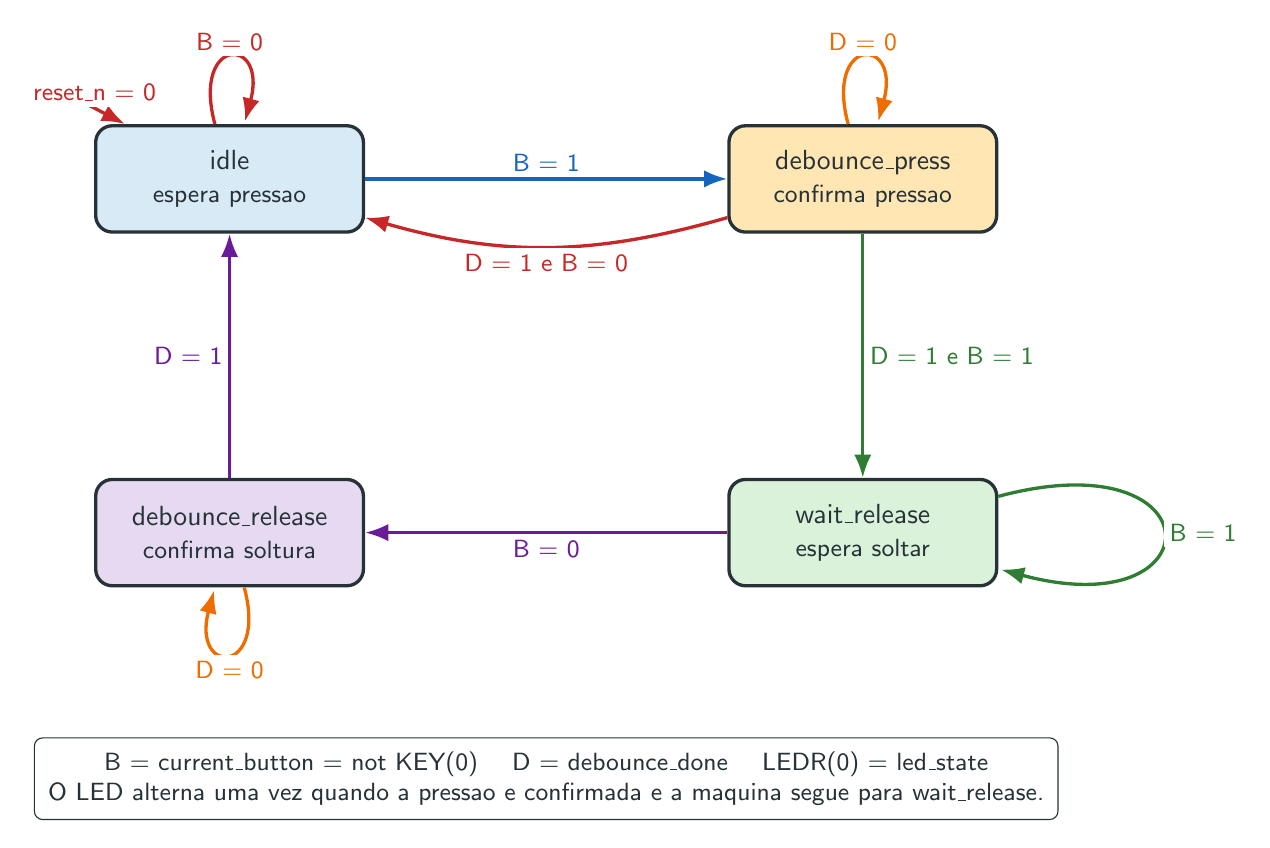
\begin{tikzpicture}[
    >=Latex,
    node distance=4.6cm,
    every node/.style={font=\sffamily},
    state/.style={
        draw=textgray,
        very thick,
        rounded corners=6pt,
        minimum width=3.4cm,
        minimum height=1.35cm,
        align=center,
        text=textgray
    },
    edge/.style={->, very thick, text=textgray},
    reset/.style={->, very thick, resetred},
    labelbox/.style={
        fill=white,
        inner sep=2pt,
        font=\sffamily\small,
        align=center
    }
]

\node[state, fill=stateidle] (idle) {idle\\{\small espera pressao}};
\node[state, fill=statepress, right=of idle] (debouncepress) {debounce\_press\\{\small confirma pressao}};
\node[state, fill=statewait, below=3.1cm of debouncepress] (waitrelease) {wait\_release\\{\small espera soltar}};
\node[state, fill=staterelease, left=of waitrelease] (debouncerelease) {debounce\_release\\{\small confirma soltura}};

\draw[reset] ($(idle)+(-2.1,1.1)$) -- node[labelbox, above, text=resetred] {reset\_n = 0} (idle);

\draw[edge, blueedge] (idle) -- node[labelbox, above] {B = 1} (debouncepress);
\path[edge, resetred] (idle) edge[loop above] node[labelbox] {B = 0} (idle);

\draw[edge, greenedge] (debouncepress) -- node[labelbox, right] {D = 1 e B = 1} (waitrelease);
\draw[edge, resetred] (debouncepress) to[bend left=16]
    node[labelbox, below] {D = 1 e B = 0} (idle);
\path[edge, orangeedge] (debouncepress) edge[loop above] node[labelbox] {D = 0} (debouncepress);

\draw[edge, purpleedge] (waitrelease) -- node[labelbox, below] {B = 0} (debouncerelease);
\path[edge, greenedge] (waitrelease) edge[loop right] node[labelbox] {B = 1} (waitrelease);

\draw[edge, purpleedge] (debouncerelease) -- node[labelbox, left] {D = 1} (idle);
\path[edge, orangeedge] (debouncerelease) edge[loop below] node[labelbox] {D = 0} (debouncerelease);

\node[
    font=\sffamily\small,
    align=center,
    text=textgray,
    draw=textgray,
    rounded corners=3pt,
    fill=white,
    inner sep=5pt,
    below=2.6cm of $(debouncerelease)!0.5!(waitrelease)$
] {
    B = current\_button = not KEY(0) \quad
    D = debounce\_done \quad
    LEDR(0) = led\_state\\
    O LED alterna uma vez quando a pressao e confirmada e a maquina segue para wait\_release.
};

\end{tikzpicture}
\end{document}
